% Digital Logic Report Template
% Created: 2020-01-10, John Miller

%==========================================================
%=========== Document Setup  ==============================

% Formatting defined by class file
\documentclass[11pt]{article}

% ---- Document formatting ----
\usepackage[margin=1in]{geometry}	% Narrower margins
\usepackage{booktabs}				% Nice formatting of tables
\usepackage{graphicx}				% Ability to include graphics

%\setlength\parindent{0pt}	% Do not indent first line of paragraphs 
\usepackage[parfill]{parskip}		% Line space b/w paragraphs
%	parfill option prevents last line of pgrph from being fully justified

% Parskip package adds too much space around titles, fix with this
\RequirePackage{titlesec}
\titlespacing\section{0pt}{8pt plus 4pt minus 2pt}{3pt plus 2pt minus 2pt}
\titlespacing\subsection{0pt}{4pt plus 4pt minus 2pt}{-2pt plus 2pt minus 2pt}
\titlespacing\subsubsection{0pt}{2pt plus 4pt minus 2pt}{-6pt plus 2pt minus 2pt}

% ---- Hyperlinks ----
\usepackage[colorlinks=true,urlcolor=blue]{hyperref}	% For URL's. Automatically links internal references.

% ---- Code listings ----
\usepackage{listings} 					% Nice code layout and inclusion
\usepackage[usenames,dvipsnames]{xcolor}	% Colors (needs to be defined before using colors)

% Define custom colors for listings
\definecolor{listinggray}{gray}{0.98}		% Listings background color
\definecolor{rulegray}{gray}{0.7}			% Listings rule/frame color

% Style for Verilog
\lstdefinestyle{Verilog}{
	language=Verilog,					% Verilog
	backgroundcolor=\color{listinggray},	% light gray background
	rulecolor=\color{blue}, 			% blue frame lines
	frame=tb,							% lines above & below
	linewidth=\columnwidth, 			% set line width
	basicstyle=\small\ttfamily,	% basic font style that is used for the code	
	breaklines=true, 					% allow breaking across columns/pages
	tabsize=3,							% set tab size
	commentstyle=\color{gray},	% comments in italic 
	stringstyle=\upshape,				% strings are printed in normal font
	showspaces=false,					% don't underscore spaces
}

% How to use: \Verilog[listing_options]{file}
\newcommand{\Verilog}[2][]{%
	\lstinputlisting[style=Verilog,#1]{#2}
}




%======================================================
%=========== Body  ====================================
\begin{document}

\title{ELC 2137 Lab 09: ALU with Input Register}
\author{Yiting Wang}

\maketitle


\section*{Summary}

Type the summary of your experiment and results here.  


\section*{Q\&A}

There is no question in the lab 09 assignment.


\section*{Results}


Firgure 1 is the simulation waveform and ERT of the register.\\
\begin{figure}[ht]\centering
	\begin{tabular}{l|rrrrrrrrrrr}
		Time (ns): & 0-5 & 5-10 & 10-15 & 15-20 & 20-25 & 25-30 & 30-35 & 35-40 & 40-45 & 45-50 & 50-55 \\
		\midrule
		D (hex) & 0 & 0 	  & A & A & 3 	    & 3 	  & 0 	    & 0 & 0$\to$6 & 6 & 6 \\
		clk     & 0 & 1 	  & 0 & 1 & 0 	    & 1 	  & 0 	    & 1 & 0 	  & 1 & 0 \\
		en  	& 0 & 0 	  & 1 & 1 & 1$\to$0 & 0$\to$1 & 1$\to$0 & 0 & 0$\to$1 & 1 & 1 \\
		rst 	& 0 & 0$\to$1 & 0 & 0 & 0 		& 0 	  & 0		& 0 & 0		  & 0 & 0 \\
		\midrule
		Q (hex) & X & X$\to$0 & 0 & a & a & a & a & a & a & 6 & 6 \\
		\bottomrule
	\end{tabular}\medskip
	
	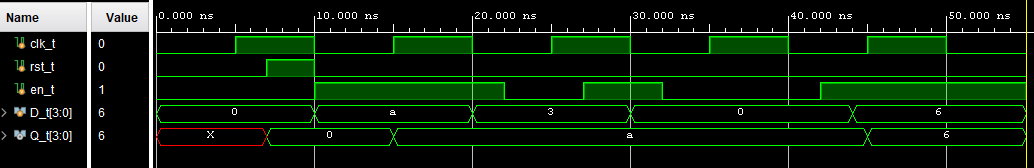
\includegraphics[width=1\textwidth]{register_simulation}
	\caption{the simulation waveform and ERT of the register}
	\label{fig:register_simulation}
\end{figure}


Firgure 2 is the simulation waveform and ERT of the ALU.\\
\begin{figure}[ht]\centering
	\begin{tabular}{l|rrrrrr}
		Time (ns): & 0-10 & 10-20 & 20-30 & 30-40 & 40-50 & 50-60 \\
		\midrule
		in0 & 1101 & 1101 & 1101 & 1101 & 1101 & 1101 \\
		in1 & 1010 & 1010 & 1010 & 1010 & 1010 & 1010 \\
		op	& 0000 & 0001 & 0010 & 0011 & 0100 & 0101 \\
		\midrule
		out & 0111 & 0011 & 1000 & 1111 & 0111 & 1101 \\
		\bottomrule
	\end{tabular}\medskip
	
	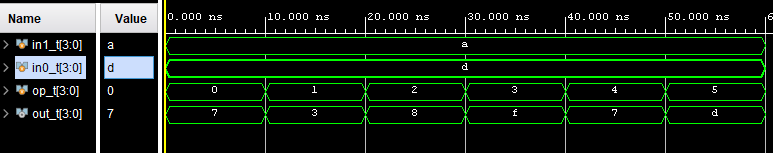
\includegraphics[width=1\textwidth]{alu_simulation}
	\caption{the simulation waveform and ERT of the ALU}
	\label{fig:alu_simulation}
\end{figure}


This is the picture of a copy of the relevant TCL Console output for Top-Level Simulation.
\begin{center}
	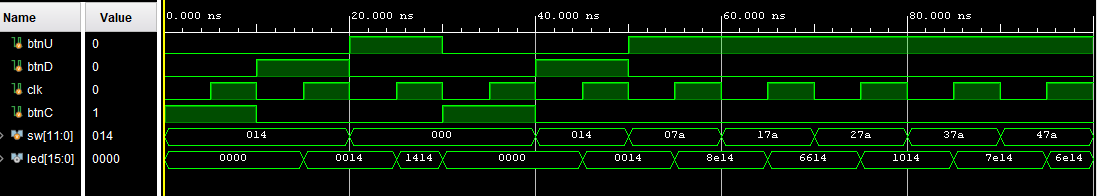
\includegraphics[width=1\textwidth]{top_level_simulation}
\end{center}


\section*{Code}


\subsection*{File Inclusion}
\Verilog[caption=mux4 Verilog code,label=code:file_ex]{register.sv}

\subsection*{File Inclusion}
\Verilog[caption=mux4 Test Benches Verilog code,label=code:file_ex]{register_test.sv}


\subsection*{File Inclusion}
\Verilog[caption=anode decoder Verilog code,label=code:file_ex]{alu.sv}

\subsection*{File Inclusion}
\Verilog[caption=anode decoder Test Benches Verilog code,label=code:file_ex]{alu_test.sv}


\subsection*{File Inclusion}
\Verilog[caption=sseg4 Verilog code,label=code:file_ex]{top_lab9.sv}




\end{document}
